\documentclass[conference]{IEEEtran}
\IEEEoverridecommandlockouts
% The preceding line is only needed to identify funding in the first footnote. If that is unneeded, please comment it out.
\usepackage{cite}
\usepackage{amsmath, amssymb, amsfonts}
\usepackage{algorithmic}
\usepackage{graphicx}
\usepackage{textcomp}
\usepackage{fourier}
%\usepackage{libertinust1math} % - cool one
\usepackage{MnSymbol}
\usepackage[english]{babel}
\usepackage[fixlanguage]{babelbib}
\usepackage[unicode=true,hidelinks]{hyperref}

\begin{document}

\renewcommand*{\figureautorefname}{Fig.}
\renewcommand*{\equationautorefname}{Eq.}

\def \w{\omega}

% ------------------------- %

\def \eq{\begin{equation}}
\def \qe{\end{equation}}
\def \eqc{\begin{equation*}}
\def \cqe{\end{equation*}}

% ------------------------- %
% ------------------------- %

\newcommand{\shifthat}[2]{%
    \stackengine{\Sstackgap}{$#2$}{\(\hspace{#1}\hat{}\)}{O}{l}{F}{T}{S}
}

% ------------------------- %

\newcommand{\operator}[2][operator]{
    \if H#2\shifthat{0.5em}{#2}\else
    \if d#2\shifthat{0.49em}{#2}\else
    \if q#2\shifthat{0.35em}{#2}\else
    \if \mu#2\shifthat{0.35em}{#2}\else
    \shifthat{0.45em}{#2}
    \fi
    \fi
    \fi
    \fi
}

% ------------------------- %

\newcommand{\vectoperator}[2][operator]{
    \if d#2\shifthat{0.367em}{\textbf{#2}}\else
    \if m#2\shifthat{0.4em}{\textbf{#2}}\else
    \shifthat{0.275em}{\textbf{#2}}
    \fi
    \fi
}

% ------------------------- %

\newcommand{\vect}[3][vector]{
    \overrightarrow{#2_{#3}}
}

% ------------------------- %

\newcommand{\vectbf}[2][bold vector]{
    \vect{\textbf{#2}}
}

% ------------------------- %

\newcommand{\pd}[3][empty]{
    \frac{\partial {#2}}{\partial {#3}}
}

% ------------------------- %

\newcommand{\func}[5][empty]{
    {#2}_{#3}^{#4} \left({#5} \right)
}

% ------------------------- %

\newcommand{\underrel}[3][]{
    \mathrel{\mathop{#3}\limits_{
        \ifx c#1\relax\mathclap{#2}\else#2\fi
    }}
}
% ------------------------- %

\makeatletter

\newcommand{\Autoref}[1]{\@first@ref#1,@}
\def\@throw@dot#1.#2@{#1}% discard everything after the dot
\def\@set@refname#1{%    % set \@refname to autoefname+s using \getrefbykeydefault
    \edef\@tmp{\getrefbykeydefault{#1}{anchor}{}}%
    \xdef\@tmp{\expandafter\@throw@dot\@tmp.@}%
    \ltx@IfUndefined{\@tmp autorefnameplural}%
        {\def\@refname{\@nameuse{\@tmp autorefname}}}%
        {\def\@refname{\@nameuse{\@tmp autorefnameplural}}}%
}
\def\@first@ref#1,#2{%
\ifx#2@\autoref{#1}\let\@nextref\@gobble% only one ref, revert to normal \autoref
\else%
    \@set@refname{#1}%  set \@refname to autoref name
    \@refname\ref{#1}% add autoefname and first reference
    \let\@nextref\@next@ref% push processing to \@next@ref
\fi%
\@nextref#2%
}
\def\@next@ref#1,#2{%
\ifx#2@,~\ref{#1}\let\@nextref\@gobble% at end: print and+\ref and stop
\else, \ref{#1}% print  ,+\ref and continue
\fi%
\@nextref#2%
}

\makeatother

% ------------------------- %
% ------------------------- %

\newcommand{\img}[4][anything]{
    \begin{figure}[H]{
        \center{\includegraphics[width={#4}]{{#1}}}
        \caption{#2}\label{#3}}
    \end{figure}
}

% ------------------------- %

\newcommand{\floatimg}[4][anything]{
    \begin{figure}[ht]{
        \center{\includegraphics[width={#4}]{{#1}}}
        \caption{#2}\label{#3}}
    \end{figure}
}

% ------------------------- %

\newcommand{\subimg}[2][anything]{
    \begin{minipage}[h]{{#2}} % 0.4\textwidth
        \center{\includegraphics[width=1\linewidth]{{#1}}}
    \end{minipage}
}

% ------------------------- %

\newcommand{\subimgtwo}[4][anything]{
    \subfloat[{#2}]{\includegraphics[width={#4}]{{#1}}\label{#3}}
}

% ------------------------- %

\title{Angular dispersion boost of high order laser harmonics interacting with dense
plasma clusters}
% {\footnotesize \textsuperscript{*}\textit{Note: Sub-titles are not captured in Xplore and
% should not be used (this footnote should be deleted)}}
% \thanks{Identify applicable funding agency here. If none, delete this.}
% }

\author{
	\IEEEauthorblockN{L.A. Litvinov\textsuperscript{1}, A.A. Andreev\textsuperscript{1, 2}}
	\IEEEauthorblockA{\textsuperscript{1}Saint Petersburg State University, Saint Petersburg, Russia}
	\IEEEauthorblockA{\textsuperscript{2}Ioffe Physico-Technical Institute, Saint Petersburg, Russia}
}


\maketitle

\begin{abstract}
	 We propose a nanosphere array target in the plasma phase as an efficient dispersive medium for the intense XUV light which is originated from laser-plasma interactions where various high harmonic generation processes take place. The scattering process is studied with the help of numerical simulations using resonance conditions obtained from the analytical model. We show that the angular distribution of different harmonics after scattering can be good described by a simple interference, in particular for the rectangle symmetry the angular distribution corresponds to the Bragg-Wolfe diffraction theory.
\end{abstract}

% \begin{IEEEkeywords}
% 	component, formatting, style, styling, insert
% \end{IEEEkeywords}

%\section{Introduction}
~\\

% Periodic surface gratings or photonic crystals are excellent tools for diffracting light and to collect information about the spectral intensity, if the target structure is known, or about the diffracting object, if the light source is well defined. However, this method is less effective in the case of extreme ultraviolet (XUV) light due to the high absorption coefficient of any material in this frequency range.

Limited size targets interacting with high-intensity coherent radiation is well-studied phenomenon of linear excited surface plasmonic oscillations. Absorption and scattering of incident light in this case good described with Mie theory predicting exist of resonance corresponding to multipole oscillations of part of the target free electrons relative to positive charged ions. Exciting of surface plasmons can lead to significant boost internal and external field on cluster eigenfrequency. In turn, this can cause enhancement of field scattered on large angles relative to the direction of incident wave.

% Unlike microwave and X-ray range, it is difficult to control XUV radiation due to the high absorption coefficient of any material in this range. 

Within the present work we consider the possibility of directed scattering of short wavelength radiation in the XUV range by scattering on suitable spherical clusters.

%\section{Base model}

Similar to the work~\cite{andreev_lecz} we develop analytical model for a single cluster based on the Drude dielectic function of the plasma and the Mie scattering theory. To investigate the conditions under which resonant field enhancement occur the determination of the scattering coefficients is necessary in general. Since we are only interested in particle sizes which are smaller than the incident wavelength we use the limiting forms of the respective Bessel functions~\cite{boren_huffman}.

%In the spherical coordinate system the solution of the scalar Helmholtz Equation can be written using spherical Bessel functions and spherical harmonics including the associated Legendre polynomial. %We can expand the incident field into series of spherical vector harmonics using generalized Fourier expantions, that allows to describe the solution with scattering coefficients~\cite{boren_huffman}.

% In the case of linear interaction Mie theory can be used for the description of elastic electromagnetic waves scattering by arbitrary sized particles and beyond that, it allows the description of the electric and magnetic field distribution inside and outside the scatter \cite{boren_huffman}. A main step is to solve the scalar Helmholtz Equation in suitable coordinate system and gain the vector solutions. For spherical cluster the solution of corresponding equation can be written in a spherical Bessel function of the $l$-th kind and $n$-th order the spherical harmonic including the associated Legendre polynomial~\cite{boren_huffman}.

% Assume an incident plane wave propagating along $z$ axis of cartesian coordinate system and polarized along $x$ axis.

% Now we can expand the plane wave into series using generalized Fourier expantions. Assuming our media is isotropic we obtain following form of scattered field~\cite{boren_huffman}:

%     \eq
% 		\vectbf{E}{s} = \sum_{n = 1}^{\infty}E_n \left[ i a_n\left(ka, m\right) \vectbf{N}{}^{(3)}_{e1n} - b_n\left(ka, m\right) \vectbf{M}{}^{(3)}_{o1n} \right]
%         \label{E_s_sph}
% 	\qe
% 	\eqc
% 		E_n = i^{n} E_0 \frac{2n + 1}{n \left(n + 1\right)}
% 	\cqe

% $n$ --- vector harmonic number after cartesian-spherical coordinate system transformation, $m = \sqrt{\varepsilon\left(\w\right)}$ --- refractive index of the target.

% Coefficients in \autoref{E_s_sph} can be described with Riccati-Bessel functions~\cite{boren_huffman}.

    % \eq
	% 	a_n(x,\:m) = \frac{m \func{\psi}{n}{\prime}{x} \func{\psi}{n}{}{mx} - \func{\psi}{n}{\prime}{mx} \func{\psi}{n}{}{x}}{m \func{\xi}{n}{\prime}{x} \func{\psi}{n}{}{mx} - \func{\psi}{n}{\prime}{mx} \func{\xi}{n}{}{x}},
	% 	\label{an_bessel}
	% \qe

    % \eq
    %     b_n(x,\:m) = \frac{\func{\psi}{n}{\prime}{x} \func{\psi}{n}{}{mx} - m \func{\psi}{n}{\prime}{mx} \func{\psi}{n}{}{x}}{\func{\xi}{n}{\prime}{x} \func{\psi}{n}{}{mx} - m \func{\psi}{n}{\prime}{mx} \func{\xi}{n}{}{x}},
    %     \label{bn_bessel}
    % \qe
	% \eqc % artificial indent after the equation
    % \cqe %

% \noindent where $\func{\psi}{n}{}{z} = z \func{j}{n}{}{z}$, $\func{\xi}{n}{}{z} = z \func{h}{n}{}{z}$ --- Riccati-Bessel functions, $h_n = j_n + i \gamma_n$ --- spherical Hankel functions of the first kind.

%\subsection{Resonance conditions}

% In zero-order Bessel functions approximation amplitude of the scattered field is maximum for $m^2 = - (n+ 1) / n$ when $ka \ll 1$, that gain corresponding set of resonance densities in collision-less case. For $ka \sim 1$ this approximation ceases to be reasonable already, so the first-order approximation is better suited \cite{abra_steg}. Moreover, in this approximation dependency of coefficients on the scatter size occurs, which lead to corresponding dependency of resonance electron density.

Such approximations allow us to estimate the resonance parameters for a target, in particular resonance electron density and radius, for pre-defined wavelength.

As we consider XUV range radiation (20-120 nm), radiuses of spherical scatters should be about few nanometers, that causes $ka \sim 1$. In first-order approximation with wavelength $\lambda_{10} = \lambda_{L} / 10 = 83$ nm, we have $n_e \approx 5.7 \cdot 10^{23}$ $\textrm{cm}^{-3}$ for $ka = 0.7$ ($a \approx 8.91$ nm) to reach efficient scattering.

%Obviously, for such $ ka $ the resonance values of the electron density can be large in considering $n = 1$ as term with the largest contribution to the scattered field. Staying within high-temperature plasma we should use only $n_e < 10^{24}$ $\textrm{cm}^{-3}$.



With these parameters of the single cluster target we consider the resonance and non-resonance case, corresponding to the 1st and 10th harmonic. We found a good scattered field enhancement (about 5 times) in the resonance case in comparison with the non-resonance case.

%\section{Simulations}

%\subsection{Scattering by an array}

Using the same resonance conditions for a single plasma cluster, we simulate diffraction by arrays of such clusters in the same cases, described by the laser and 10th harmonic, using code CELES~\cite{celes}. 
% Simple cubic lattice with different grating constant $d$ is considered spatial configuration of a volume grating.


% ------------------------

% Diffraction orders can be obtained with Bragg's law \cite{kress_bernard}.

% According to Bragg's law we obtain $\theta = \arcsin\frac{1}{4}$ for grating with $d = 2\lambda$ and $\theta = \arcsin\frac{1}{6}$ for grating with $d = 3\lambda$ in $1$-st diffraction order. Using these values we numerically compute the scattered field of 10-th laser harmonic with wavelength $\lambda_{10} = 83$ nm.

% We can see directions corresponding to the angular boost of the incident beam, in particular, for $d = 2\lambda_{10}$ there are two fairly clear directions.

\begin{figure}[htbp]
	\centerline{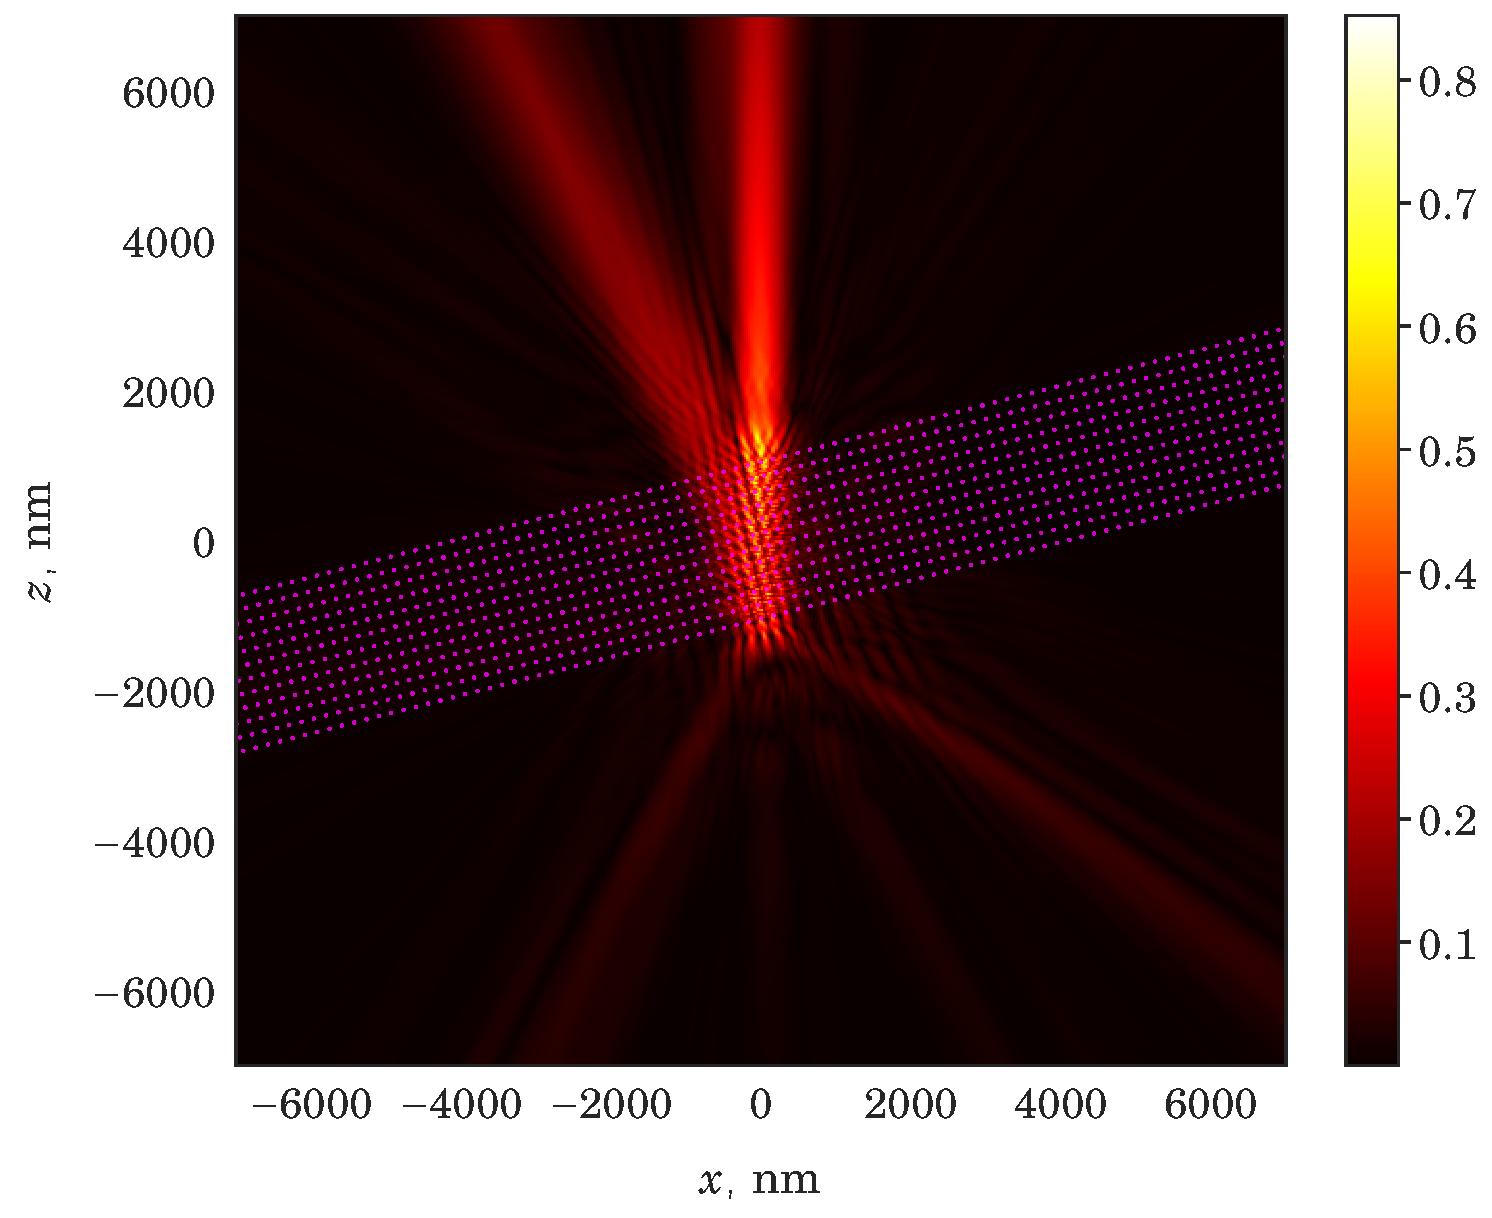
\includegraphics[width=0.84\columnwidth]{../components/img/celes/TE_14.324deg_check.pdf}}
	\caption{Scattered electric field normalized by the incident beam amplitude. The incident field represented by the gaussian beam with width $w = 300$ nm, $x$-polarized, propagating along positive direction of $z$ axis; the incident angle $\theta = 14.324^{\circ}$, the distance between clusters $d = 2\lambda_{10}$.}
	\label{14.324deg:image}
\end{figure}

%\section*{Conclusion}

Obtained results show a significant boost of the scattered field in the resonance case for large angles, which corresponds to the Bragg-Wolfe diffraction theory~\cite{boren_huffman}, --- the ability to control high harmonics of laser radiation (XUV range) using an ionized cluster gas.

\selectbiblanguage{english}
\bibliographystyle{ieeetr}
\bibliography{../components/bibliography.bib}

\end{document}
